\section{Das semantische Datenmodell}

Die Notwendigkeit für semantische Datenmodelle wurde erstmals Mitte der 70er Jahre von der US-amerikanischen Luftwaffe als Ergebnis des Programms "Integrated Computer-Aided Manufacturing" (ICAM) erkannt. Ziel dieses Programms war es, die Fertigungsproduktivität durch die systematische Anwendung der Computertechnik zu erhöhen. Das ICAM-Programm ermittelte einen Bedarf an besseren Analysen- und Kommunikationstechniken für Personen, die an der Verbesserung der Fertigungsproduktivität beteiligt waren. Infolgedessen entwickelte das ICAM-Programm eine Reihe von Techniken, die als IDEF (ICAM Definition) Methoden bekannt sind. \cite{bekke2005} Es gab die folgenden Methoden:
IDEF0 wurde verwendet, um ein "Funktionsmodell" zu erstellen, das eine strukturierte Darstellung der Aktivitäten oder Prozesse innerhalb der Umgebung oder des Systems ist.
IDEF1 wurde verwendet, um ein "Informationsmodell" zu produzieren, das die Struktur und die Semantik von Informationen innerhalb der Umgebung oder des Systems darstellt.
IDEF1X war eine semantische Datenmodellierungstechnik. Es wurde verwendet, um ein grafisches Informationsmodell zu erzeugen, das die Struktur und die Semantik von Informationen innerhalb einer Umgebung oder eines Systems darstellt. Die Verwendung dieses Standards erlaubt den Aufbau von semantischen Datenmodellen, die dazu dienen können, das Management von Daten als Ressource, die Integration von Informationssystemen und den Aufbau von Computerdatenbanken zu unterstützen.
IDEF2 wurde verwendet, um ein "Dynamikmodell" zu produzieren, das die zeitvariablen Verhaltensmerkmale der Umgebung oder des Systems darstellt \cite{rishe1992}.
In den 1990er Jahren führte die Anwendung semantischer Modellierungstechniken zu den semantischen Datenmodellen der zweiten Art. Ein Beispiel dafür ist das semantische Datenmodell, das als ISO 15926-2 (2002) standardisiert ist und in die semantische Modellierungssprache Gellish (2005) weiterentwickelt wird. Die Definition der Gellish-Sprache ist in Form eines semantischen Datenmodells dokumentiert. Gellish selbst ist eine semantische Modellierungssprache, die verwendet werden kann, um andere semantische Modelle zu erstellen. Diese semantischen Modelle können in Gellish Datenbanken gespeichert werden, wobei es sich um semantische Datenbanken handelt. \cite{gray2004}
Das semantische Datenmodell ist eine Methode zur Strukturierung von Daten, um es in einer bestimmten logischen Weise darzustellen. Es handelt sich um ein konzeptionelles Datenmodell, das semantische Informationen enthält, die den Daten und den zwischen ihnen liegenden Beziehungen eine grundlegende Bedeutung verleihen. Dieser Ansatz zur Datenmodellierung und Datenorganisation ermöglicht die einfache Entwicklung von Anwendungsprogrammen und auch für die einfache Pflege der Datenkonsistenz bei der Aktualisierung der Daten.
Das semantische Datenmodell ist ein relativ neuer Ansatz, der auf semantischen Prinzipien basiert.  In der Regel, Singular-Daten oder ein Wort vermittelt keine Bedeutung für den Menschen, aber verbundet mit einem Kontext erbt dieses Wort mehr Bedeutung.
In einer Datenbankumgebung wird der Kontext von Daten oft hauptsächlich durch seine Struktur, wie seine Eigenschaften und Beziehungen mit anderen Objekten definiert. So wird in einem relationalen Ansatz die vertikale Struktur der Daten durch explizite referentielle Einschränkungen definiert, aber bei der semantischen Modellierung wird diese Struktur in einer inhärenten Weise definiert. \cite{hammer2008}
Typischerweise enthalten die Instanzdaten von semantischen Datenmodellen explizit die Beziehungen zwischen den verschiedenen Datenelementen, wie z. B. <befindet sich in>. Um die Bedeutung der Tatsachen aus den Instanzen zu interpretieren, ist es erforderlich, die Bedeutung der Arten von Beziehungen (Relationstypen) zu kennen. Daher standardisieren semantische Datenmodelle typischerweise solche Relationstypen. Die zweite Art von semantischen Datenmodellen erstellen in der Regel semantische Datenbanken. Die Möglichkeit, die Bedeutung in semantischen Datenbanken einzubeziehen, erleichtert den Aufbau verteilter Datenbanken, die ermöglichen die Bedeutung aus dem Inhalt zu interpretieren. Dies bedeutet, dass semantische Datenbanken integriert werden können, wenn sie dieselben (Standard-) Relationstypen verwenden. Dies bedeutet auch, dass sie im Allgemeinen eine breitere Anwendbarkeit als relationale oder objektorientierte Datenbanken haben. \cite{bekke2005}
Ein semantisches Datenmodell kann grafisch durch ein Abstraktionshierarchiediagramm dargestellt werden, das Datentypen als Felder und deren Beziehungen als Linien anzeigt. Dies geschieht hierarchisch, so dass Typen, die auf andere Typen verweisen, immer über den Typen aufgeführt sind, auf die sie verweisen. Das macht es leichter zu lesen und zu verstehen. \cite{hammer2008}
In einem semantischen Datenmodell verwendet man die Abstraktionen:
Klassifizierung - "{}instance\_of"{} Beziehungen
Aggregation - "{}has\_a"{} Beziehungen
Verallgemeinerung - "{}is\_a"{} Beziehungen
Die logische Datenstruktur eines Datenbankmanagementsystems (DBMS), ob hierarchisch, netz oder relational, kann die Voraussetzungen für eine konzeptionelle Definition von Daten nicht vollständig erfüllen, da sie im Umfang begrenzt und auf die Implementierungsstrategie des DBMS angewiesen ist. Daher die Notwendigkeit Daten aus einer konzeptionellen Sicht zu definieren, hat zur Entwicklung von semantischen Datenmodellierungstechniken geführt. Das heißt, Techniken, um die Bedeutung von Daten im Kontext ihrer Zusammenhänge mit anderen Daten zu definieren. Wie in der Abbildung dargestellt, die reale Welt, in Bezug auf Ressourcen, Ideen, Ereignisse, etc., ist symbolisch in physischen Datenspeichern definiert. Ein semantisches Datenmodell ist eine Abstraktion, die definiert, wie sich die gespeicherten Symbole auf die reale Welt beziehen. So muss das Modell eine wahre Darstellung der realen Welt sein. \cite{bekke2005}

\begin{figure}[htp]
\centering
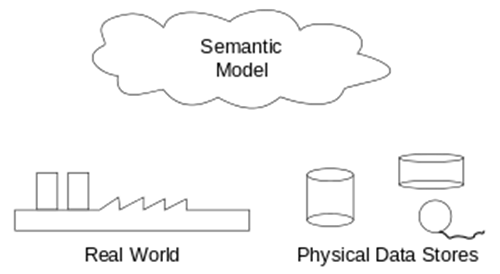
\includegraphics[width=0.7\textwidth]{images/SemanticModel.png}
\caption{Sematisches Modell nach \cite{rishe1992}}
\label{oo-example}
\end{figure}


Nach Klas und Schrefl (1995) ist das "{}Ziel der semantischen Datenmodelle"{} die Erfassung von mehr Bedeutung von Daten durch die Integration von relationalen Konzepten mit leistungsstärkeren Abstraktionskonzepten, die aus dem Künstlichen Intelligenzfeld bekannt sind, zu erfassen. Die Idee besteht darin, hochrangige Modellierungsteile als integraler Bestandteil eines Datenmodells zu erstellen, um die Darstellung von realen Weltsituationen zu erleichtern.
Semantisches Datenmodell unterscheidet sich von anderen Datenmodellen jedoch dadurch, dass es auf die Bereitstellung von der Bedeutung der Daten selbst konzentriert, anstatt nur oder primär auf die Beziehungen und Attribute der Daten.
Semantisches Datenmodell bietet ein hochrangiges Verständnis der Daten, indem es weiter weg von den physikalischen Aspekten der Datenspeicherung abstrakt. \cite{bekke2005}
Ein semantisches Datenmodell kann für viele Zwecke verwendet werden. Einige wichtige Ziele sind:
Planung von Datenressourcen: Ein vorläufiges Datenmodell kann verwendet werden, um eine Gesamtansicht der Daten zu liefern, die für die Ausführung eines Unternehmens erforderlich sind. Das Modell kann dann analysiert werden, um Projekte zu identifizieren und zu skalieren, um gemeinsam genutzte Datenressourcen zu erstellen.
Aufbau von Shared-Datenbanken: Ein voll entwickeltes Modell kann verwendet werden, um eine anwendungsunabhängige Ansicht von Daten zu definieren, die von Benutzern validiert und dann in eine physikalische Datenbankgestaltung für eine der verschiedenen DBMS-Technologien umgewandelt werden kann. Neben der Generierung von Datenbanken, die konsistent und gemeinsam genutzt werden, können die Entwicklungskosten durch Datenmodellierung drastisch reduziert werden \cite{rishe1992}.
Auswertung der Vendor-Software: Da ein Datenmodell tatsächlich die Infrastruktur einer Organisation repräsentiert, kann die Vendor-Software gegen das Datenmodell eines Unternehmens ausgewertet werden, um mögliche Inkonsistenzen zwischen der implizierten Infrastruktur und der Art und Weise, wie das Unternehmen tatsächlich tätig ist, zu identifizieren.
Integration bestehender Datenbanken: Durch die Definition der Inhalte existierender Datenbanken mit semantischen Datenmodellen kann eine integrierte Datendefinition abgeleitet werden. Mit der richtigen Technologie kann das resultierende Konzeptschema verwendet werden, um die Transaktionsverarbeitung in einer verteilten Datenbankumgebung zu steuern. Das U.S. Air Force Integrated Information Support System (I2S2) ist eine experimentelle Entwicklung und Demonstration von Technologie dieser Art, die auf eine heterogene DBMS-Umgebung angewendet wird. \cite{gray2004}
Semantische Datenelemente sind ähnlich wie die Entitäten und Attribute, die wir in einem logischen oder physikalischen Datenmodell finden, wie zum Beispiel "{}Kunde"{}, "{}Produkt"{}, "{}Kreditlimit"{}, "{}Netzwerk Verkäufe"{} und so weiter. Was der semantische Modellierer jedoch ansprechen muss, ist der Kontext des Begriffs, des Datenelements und wie er sich auf die in den Rechensystemdaten vorhandenen Datenelemente bezieht. Zum Beispiel ist ein Kunde ein Einzelner - der Einkaufsagent - oder ein Unternehmen? Was in einigen Kontexten vielleicht als "{}Perspektive"{} bezeichnet werden könnte, könnte in anderen als "{}Kunde"{} bezeichnet werden. Ist ein Kunde ein Großhändler oder ist er der Endverbraucher? Ist der Großhändler Kunde auch Kunde genannt? Die Antwort auf diese Fragen ist wahrscheinlich "{}es hängt davon ab."{} Und das ist die richtige Antwort, denn es hängt davon ab. Es hängt davon ab, wer fragt und warum. Die Verkaufsabteilung von einer Gesellschaft kann eine klare Linie zwischen Kunden (Käufer) und Interessenten machen. 
Der semantische Modellierer muss bohren und die Nuance jeder Perspektive erfassen und muss kämpfen, um mit den Geschäftsbenutzern zu arbeiten, um eine Namenskonvention oder Syntax zu entwickeln, die Klarheit bietet. Alle Perspektiven sind im semantischen Modell dargestellt. \cite{hammer2008}

